\documentclass[crop,tikz,convert={outext=.svg,command=\unexpanded{pdf2svg \infile\space\outfile}},multi=false]{standalone}
% This file is used to globally define colors, line widths, etc. for diagrams used in the thesis
\usepackage[intlimits]{amsmath}
\usepackage{amssymb}
\usepackage{tikz}
\usepackage{ifthen}
\usepackage{tikz-network}
\usepackage{pgfplots}
\pgfplotsset{compat=1.18}
\usepgfplotslibrary{colorbrewer}
\let\Re\relax
\DeclareMathOperator{\Re}{Re}
\DeclareMathOperator{\Tr}{Tr}

% Libraries
\usetikzlibrary{decorations.markings}
\usetikzlibrary{arrows}
\usetikzlibrary{positioning}
\usetikzlibrary{calc}

% Basic colors
\definecolor{borderColor}{rgb}{0.0, 0.0, 0.0}
\definecolor{physicalTensorColor}{rgb}{0.0, 0.0, 0.0}
\definecolor{auxillaryTensorColor}{rgb}{1.0, 0.0, 0.0}
\definecolor{orthogonalityCenterColor}{rgb}{1.0, 0.616, 0.0}
\definecolor{physicalLegColor}{rgb}{0.5, 0.5, 0.5}
\definecolor{auxillaryLegColor}{rgb}{1.0, 0.0, 0.0}
\definecolor{virtualLegColor}{rgb}{0.0, 0.0, 0.0}
\definecolor{generalTensorColor}{rgb}{0.757, 0.827, 0.996}
\definecolor{identityColor}{rgb}{1.0, 1.0, 1.0}
\definecolor{redMarkingColor}{rgb}{1.0, 0.0, 0.0}
\definecolor{greenMarkingColor}{rgb}{0.1, 0.8, 0.1}
\definecolor{operatorColor}{rgb}{0.5, 1.0, 0.5}
\definecolor{specialLegColor}{HTML}{5d3fd3}
\definecolor{toricCodeSpinColor}{rgb}{1.0, 0.0, 0.0}
\definecolor{toricCodeEdgeSpinColor}{rgb}{0.0, 0.0, 0.7}
\definecolor{toricCodeAOperatorColor}{rgb}{0.0, 0.8, 0.0}
\definecolor{toricCodeBOperatorColor}{rgb}{0.0, 0.0, 1.0}
\definecolor{toricCodeDisoTPSTensorColor}{HTML}{5d3fd3}
\def \backgroundopacity {0.5}

\definecolor{color1}{HTML}{3182bd} % Same as 5blue4
\definecolor{color2}{HTML}{fd8d3c} % Same as 5orange3
\definecolor{color3}{HTML}{31a354} % Same as 5green4
\definecolor{color4}{HTML}{a50f15} % Same as 5red5

% Basic sizes
\def \defaultTensorWidth {19pt}
\def \smallTensorWidth {13pt}
\def \tinyTensorWidth {4pt}
\def \defaultLineWidth {2}
\def \lineWidthThick {2.5}
\def \lineWidthThin {1.8}
\def \lineWidthTiny {1.2}
\def \lineWidthHuge {4}
\def \xOffsetUnitCell {180pt}
\def \yOffsetUnitCell {180pt}
\def \yOffsetPhysicalLeg {30pt}
\def \physicalLegLength {30pt}
\def \physicalLegLengthSmall {15pt}
\def \defaultArrowscale {0.7}
\def \arrowScaleSmall {0.6}
\def \defaultArrowXShift {7pt}
\def \defaultDoubleArrowXShift {5pt}
\def \defaultTextOffset {6pt}
\def \defaultTextOffsetLarge {9pt}
\def \defaultTextOffsetSmall {1pt}
\def \defaultDistanceSmall {30pt}
\def \defaultDistanceSmallDiagonal {32pt}
\def \defaultDistanceNormal {40pt}
\def \defaultDistanceLarge {62 pt}
\def \defaultDistanceEquations {40pt}
\def \identityLegDistance {10 pt}
\def \isoTPSPhysicalLegAngle {30}
\def \defaultLegSeperationSmall{4pt}
\def \defaultLegSeperation{6.5pt}
\def \defaultLegSeperationLarge{9pt}
\def \roundedCornerInsetNormal{10pt}
\def \roundedCornerInsetSmall{2pt}
\def \braceWidth{10pt}
\def \physicalLegLengthSmallMPS{1.3*\physicalLegLengthSmall}


\def\tensorDistanceMPS{1.2*\defaultDistanceSmall}
\def\braketDistanceMPS{1.2*\defaultDistanceNormal}
\def\tensorWidthMPS{\smallTensorWidth}
\def\openLegMultiplierMPS{0.9}

% Tensor styles
\tikzstyle{tensorPhysical} = [circle, minimum size=\defaultTensorWidth, line width=\defaultLineWidth, fill=physicalTensorColor, draw=borderColor, outer sep=0]
\tikzstyle{tensorAuxillary} = [circle, minimum size=\defaultTensorWidth, line width=\defaultLineWidth, fill=auxillaryTensorColor, draw=borderColor, outer sep=0]
\tikzstyle{tensorOrthoCenter} = [circle, minimum size=\defaultTensorWidth, line width=\defaultLineWidth, fill=orthogonalityCenterColor, draw=borderColor, outer sep=0]

\tikzstyle{tensorPhysicalSmall} = [circle, minimum size=\smallTensorWidth, line width=\defaultLineWidth, fill=physicalTensorColor, draw=borderColor, outer sep=0]
\tikzstyle{tensorAuxillarySmall} = [circle, minimum size=\smallTensorWidth, line width=\defaultLineWidth, fill=auxillaryTensorColor, draw=borderColor, outer sep=0]
\tikzstyle{tensorOrthoCenterSmall} = [circle, minimum size=\smallTensorWidth, line width=\defaultLineWidth, fill=orthogonalityCenterColor, draw=borderColor, outer sep=0]

\tikzstyle{tensorOperator} = [rectangle, line width=\defaultLineWidth, fill=operatorColor, draw=borderColor, rounded corners=\roundedCornerInsetNormal]
\tikzstyle{tensorOperatorSmall} = [rectangle, line width=\defaultLineWidth, fill=operatorColor, draw=borderColor, rounded corners=\roundedCornerInsetSmall]

\tikzstyle{toricCodeSpin} = [circle, minimum size=\tinyTensorWidth, line width=\defaultLineWidth, fill=toricCodeSpinColor, draw=toricCodeSpinColor, inner sep=0, outer sep=0]
\tikzstyle{toricCodeEdgeSpin} = [circle, minimum size=\tinyTensorWidth, line width=\defaultLineWidth, fill=toricCodeEdgeSpinColor, draw=toricCodeEdgeSpinColor, inner sep=0, outer sep=0]
\tikzstyle{toricCodePEPSCenterTensor} = [circle, minimum size=2*\tinyTensorWidth, line width=\defaultLineWidth, fill=physicalTensorColor, draw=physicalTensorColor, inner sep=0, outer sep=0]
\tikzstyle{toricCodeDisoTPSTensor} = [circle, minimum size=0.9*\defaultTensorWidth, line width=\defaultLineWidth, fill=toricCodeDisoTPSTensorColor, draw=physicalTensorColor, inner sep=0, outer sep=0]

\tikzstyle{tensorPhysicalMPS} = [circle, minimum size=\smallTensorWidth, line width=\defaultLineWidth, fill=generalTensorColor, draw=borderColor, outer sep=0]
\tikzstyle{tensorPhysicalMPSCanonical} = [circle, minimum size=\smallTensorWidth, line width=\defaultLineWidth, fill=physicalTensorColor, draw=borderColor, outer sep=0]
\tikzstyle{tensorPhysicalMPSCanonicalOrthoCenter} = [circle, minimum size=\smallTensorWidth, line width=\defaultLineWidth, fill=orthogonalityCenterColor, draw=borderColor, outer sep=0]

% Leg styles
\tikzstyle{auxillaryLeg} = [color=auxillaryLegColor, line width=\defaultLineWidth, decoration={markings, mark=at position 0.5 with {\pgftransformscale{\defaultArrowscale}\arrow[xshift=\defaultArrowXShift]{triangle 60}}}, postaction={decorate}]
\tikzstyle{physicalLeg} = [color=physicalLegColor, line width=\defaultLineWidth, decoration={markings, mark=at position 0.5 with {\pgftransformscale{\defaultArrowscale}\arrow[xshift=\defaultArrowXShift]{triangle 60}}}, postaction={decorate}]
\tikzstyle{virtualLeg} = [color=virtualLegColor, line width=\defaultLineWidth, decoration={markings, mark=at position 0.5 with {\pgftransformscale{\defaultArrowscale}\arrow[xshift=\defaultArrowXShift]{triangle 60}}}, postaction={decorate}]
\tikzstyle{specialLeg} = [color=specialLegColor, line width=\defaultLineWidth, decoration={markings, mark=at position 0.5 with {\pgftransformscale{\defaultArrowscale}\arrow[xshift=\defaultArrowXShift]{triangle 60}}}, postaction={decorate}]

\tikzstyle{virtualLegLateArrows} = [color=virtualLegColor, line width=\defaultLineWidth, decoration={markings, mark=at position 0.8 with {\pgftransformscale{\defaultArrowscale}\arrow[xshift=\defaultArrowXShift]{triangle 60}}}, postaction={decorate}]
\tikzstyle{virtualLegWithoutArrows} = [color=virtualLegColor, line width=\defaultLineWidth]
\tikzstyle{physicalLegWithoutArrows} = [color=physicalLegColor, line width=\defaultLineWidth]
\tikzstyle{specialLegWithoutArrows} = [color=specialLegColor, line width=\defaultLineWidth]
\tikzstyle{virtualLegDoubleArrow} = [color=virtualLegColor, line width=\defaultLineWidth, decoration={markings, mark=at position 0.5 with {\pgftransformscale{\defaultArrowscale}\arrow[xshift=\defaultDoubleArrowXShift]{Rays[round]}}}, postaction={decorate}]
\tikzstyle{auxillaryLegWithoutArrows} = [color=auxillaryLegColor, line width=\defaultLineWidth]

\tikzstyle{auxillaryLegSmall} = [color=auxillaryLegColor, line width=\lineWidthThin, decoration={markings, mark=at position 0.5 with {\pgftransformscale{\arrowScaleSmall}\arrow[xshift=\defaultArrowXShift]{triangle 60}}}, postaction={decorate}]
\tikzstyle{auxillaryLegSmallWithoutArrows} = [color=auxillaryLegColor, line width=\lineWidthThin]
\tikzstyle{auxillaryLegSmallDoubleArrows} = [color=auxillaryLegColor, line width=\lineWidthThin, decoration={markings, mark=at position 0.5 with {\pgftransformscale{\arrowScaleSmall}\arrow[xshift=\defaultDoubleArrowXShift]{Rays[round]}}}, postaction={decorate}]
\tikzstyle{physicalLegSmall} = [color=physicalLegColor, line width=\lineWidthThin, decoration={markings, mark=at position 0.5 with {\pgftransformscale{\arrowScaleSmall}\arrow[xshift=\defaultArrowXShift]{triangle 60}}}, postaction={decorate}]
\tikzstyle{virtualLegSmall} = [color=virtualLegColor, line width=\lineWidthThin, decoration={markings, mark=at position 0.5 with {\pgftransformscale{\arrowScaleSmall}\arrow[xshift=\defaultArrowXShift]{triangle 60}}}, postaction={decorate}]
\tikzstyle{virtualLegSmallWithoutArrows} = [color=virtualLegColor, line width=\lineWidthThin]
\tikzstyle{physicalLegSmallWithoutArrows} = [color=physicalLegColor, line width=\lineWidthThin]
\tikzstyle{virtualLegSmallDoubleArrows} = [color=virtualLegColor, line width=\lineWidthThin, decoration={markings, mark=at position 0.5 with {\pgftransformscale{\arrowScaleSmall}\arrow[xshift=\defaultDoubleArrowXShift]{Rays[round]}}}, postaction={decorate}]

% special symbols
\usepackage{amssymb}
\DeclareMathAlphabet{\mathbbb}{U}{bbold}{m}{n}
\newcommand{\id}{\mathbbb{1}}
\newcommand{\iu}{\mathrm{i}}% imaginary unit number i
\newcommand{\Stiefel}{\text{St}(n,p)}


% Layers
\pgfdeclarelayer{bg} % declare background layer
\pgfsetlayers{bg,main} % set order of layers

% Command for drawing convex hulls
\newcommand{\convexhull}[2]{
	[   
	create hullnodes/.code={
		\global\edef\namelist{#1}
		\foreach [count=\counter] \nodename in \namelist {
			\global\edef\numberofnodes{\counter}
			\node at (\nodename) [draw=none,name=hullnode\counter] {};
		}
		\node at (hullnode\numberofnodes) [name=hullnode0,draw=none] {};
		\pgfmathtruncatemacro\lastnumber{\numberofnodes+1}
		\node at (hullnode1) [name=hullnode\lastnumber,draw=none] {};
	},
	create hullnodes
	]
	($(hullnode1)!#2!-90:(hullnode0)$)
	\foreach [
	evaluate=\currentnode as \previousnode using \currentnode-1,
	evaluate=\currentnode as \nextnode using \currentnode+1
	] \currentnode in {1,...,\numberofnodes} {
		-- ($(hullnode\currentnode)!#2!-90:(hullnode\previousnode)$)
		let \p1 = ($(hullnode\currentnode)!#2!-90:(hullnode\previousnode) - (hullnode\currentnode)$),
		\n1 = {atan2(\y1,\x1)},
		\p2 = ($(hullnode\currentnode)!#2!90:(hullnode\nextnode) - (hullnode\currentnode)$),
		\n2 = {atan2(\y2,\x2)},
		\n{delta} = {-Mod(\n1-\n2,360)}
		in 
		{arc [start angle=\n1, delta angle=\n{delta}, radius=#2]}
	}
	-- cycle
}

% Command for drawing braces
%% https://tex.stackexchange.com/questions/55068/is-there-a-tikz-equivalent-to-the-pstricks-ncbar-command
\tikzset{
	ncbar angle/.initial=90,
	ncbar/.style={
		to path=(\tikztostart)
		-- ($(\tikztostart)!#1!\pgfkeysvalueof{/tikz/ncbar angle}:(\tikztotarget)$)
		-- ($(\tikztotarget)!($(\tikztostart)!#1!\pgfkeysvalueof{/tikz/ncbar angle}:(\tikztotarget)$)!\pgfkeysvalueof{/tikz/ncbar angle}:(\tikztostart)$)
		-- (\tikztotarget)
	},
	ncbar/.default=0.5cm,
}

\tikzset{square left brace/.style={ncbar=10pt}}
\tikzset{square right brace/.style={ncbar=-10pt}}

\tikzset{round left paren/.style={ncbar=10pt,out=120,in=-120}}
\tikzset{round right paren/.style={ncbar=10pt,out=60,in=-60}}

% PLOTS
\RequirePackage{pgfplots}
\pgfplotsset{compat=1.18}
\usepgfplotslibrary{colorbrewer}
\RequirePackage{tikz}
% A single subfigure
\def\singleFigureWidth{8 cm}
\def\singleFigureHeight{4.944 cm}
\def\insetFigureWidth{4 cm}
\def\insetFigureHeight{2.2 cm}
% Two subfigures stacked ontop of each other
\def\doubleVerticalFigureWidth{11 cm}
\def\doubleVerticalFigureHeight{5 cm}

% 3 subfigures on top of each other
\def\tripleVerticalFigureWidth{11 cm}
\def\tripleVerticalFigureHeight{4 cm}

% 4 subfigures aranged in a 2x2 pattern
\def\twoByTwoFigureWidth{6.75cm}
\def\twoByTwoFigureHeight{4.1717cm}

% 4 subfigures side by side on one page
\def\gsEnergyVsDtauFigureWidth{3.2cm}
\def\gsEnergyVsDtauFigureHeight{4cm}

% 3 lengthy subfigures below each other
\def\globalQuenchLargeFieldFigureWidth{10cm}
\def\globalQuenchLargeFieldFigureHeight{3cm}

\def\legendscale{1.0}

\def\doubleFigureWidth{6.125cm}
\def\doubleFigureHeight{4.635cm}
% PLOT Colors
\definecolor{7blue1}{HTML}{eff3ff}
\definecolor{7blue2}{HTML}{c6dbef}
\definecolor{7blue3}{HTML}{9ecae1}
\definecolor{7blue4}{HTML}{6baed6}
\definecolor{7blue5}{HTML}{4292c6}
\definecolor{7blue6}{HTML}{2171b5}
\definecolor{7blue7}{HTML}{084594}

\definecolor{5blue1}{HTML}{eff3ff}
\definecolor{5blue2}{HTML}{bdd7e7}
\definecolor{5blue3}{HTML}{6baed6}
\definecolor{5blue4}{HTML}{3182bd}
\definecolor{5blue5}{HTML}{08519c}

\definecolor{3blue1}{HTML}{6baed6}
\definecolor{3blue2}{HTML}{3182bd}
\definecolor{3blue3}{HTML}{08519c}

\definecolor{5orange1}{HTML}{feedde}
\definecolor{5orang2}{HTML}{fdbe85}
\definecolor{5orange3}{HTML}{fd8d3c}
\definecolor{5orange4}{HTML}{e6550d}
\definecolor{5orange5}{HTML}{a63603}

\definecolor{5red1}{HTML}{fee5d9}
\definecolor{5red2}{HTML}{fcae91}
\definecolor{5red3}{HTML}{fb6a4a}
\definecolor{5red4}{HTML}{de2d26}
\definecolor{5red5}{HTML}{a50f15}

\definecolor{3red1}{HTML}{fb6a4a}
\definecolor{3red2}{HTML}{de2d26}
\definecolor{3red3}{HTML}{a50f15}

\definecolor{4red1}{HTML}{fee5d9}
\definecolor{4red2}{HTML}{fcae91}
\definecolor{4red3}{HTML}{fb6a4a}
\definecolor{4red4}{HTML}{cb181d}

\definecolor{5green1}{HTML}{edf8e9}
\definecolor{5green2}{HTML}{bae4b3}
\definecolor{5green3}{HTML}{74c476}
\definecolor{5green4}{HTML}{31a354}
\definecolor{5green5}{HTML}{006d2c}

\definecolor{5gray1}{HTML}{f7f7f7}
\definecolor{5gray2}{HTML}{cccccc}
\definecolor{5gray3}{HTML}{969696}
\definecolor{5gray4}{HTML}{636363}
\definecolor{5gray5}{HTML}{252525}

\definecolor{5purple1}{HTML}{f2f0f7}
\definecolor{5purple2}{HTML}{cbc9e2}
\definecolor{5purple3}{HTML}{9e9ac8}
\definecolor{5purple4}{HTML}{756bb1}
\definecolor{5purple5}{HTML}{54278f}

\definecolor{singleBlue}{HTML}{3182bd} % Same as 5blue4
\definecolor{singleOrange}{HTML}{fd8d3c} % Same as 5orange3
\definecolor{singleGreen}{HTML}{31a354} % Same as 5green4
\definecolor{singleRed}{HTML}{a50f15} % Same as 5red5

% axis style, ticks, etc
\pgfplotsset{every axis/.append style={
		label style={font=\small},
		tick label style={font=\small}}}

\begin{document}
	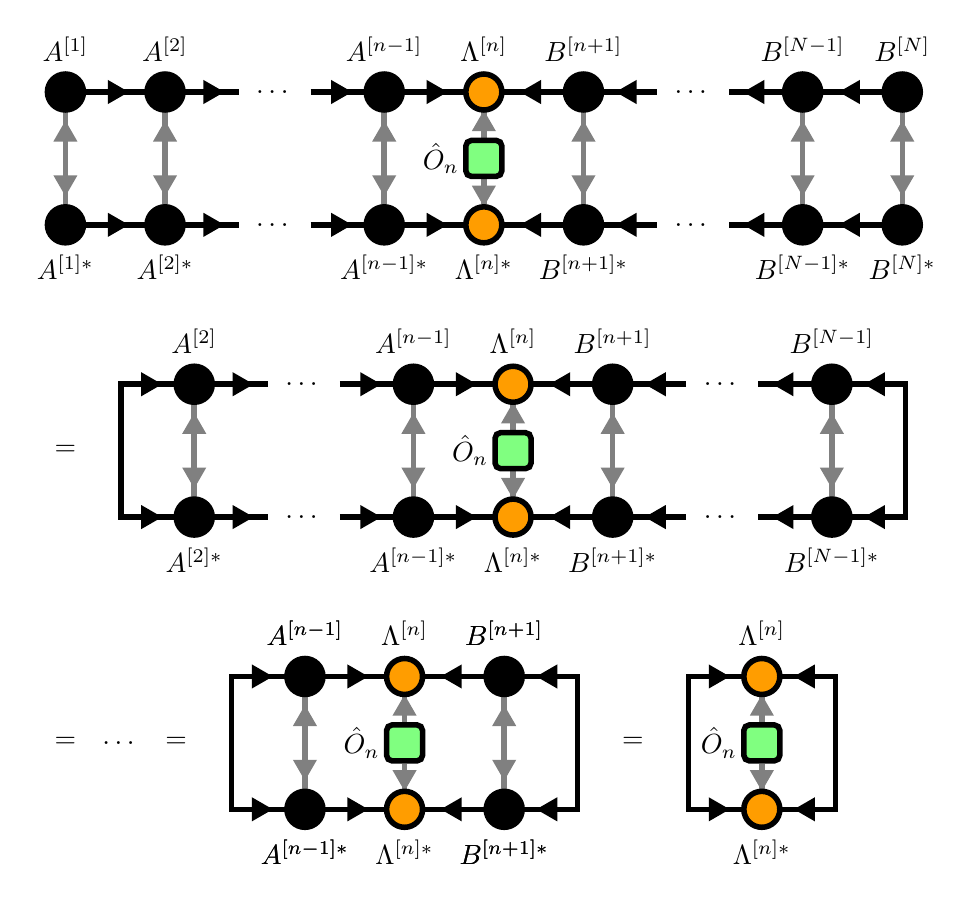
\begin{tikzpicture}
		\def\verticalLineMultiplier{2.2}
		\def\secondLineXOffset{\defaultDistanceEquations/2+\tensorDistanceMPS*\openLegMultiplierMPS-\tensorWidthMPS/2*\openLegMultiplierMPS}
		\def\thirdLineXOffsetA{3*\defaultDistanceEquations/2+\tensorDistanceMPS*\openLegMultiplierMPS-\tensorWidthMPS/2*\openLegMultiplierMPS}
		\def\thirdLineXOffsetB{5*\defaultDistanceEquations/2+2*\tensorDistanceMPS+3*\tensorDistanceMPS*\openLegMultiplierMPS-3*\tensorWidthMPS/2*\openLegMultiplierMPS}
		
		% First line
		\node[tensorPhysicalMPSCanonical] (A1) at (0, 0) {};
		\node[tensorPhysicalMPSCanonical] (A2) at (\tensorDistanceMPS, 0) {};
		\node[] () at (2.1*\tensorDistanceMPS, 0) {$\dots$};
		\node[tensorPhysicalMPSCanonical] (Anm1) at (3.2*\tensorDistanceMPS, 0) {};
		\node[tensorPhysicalMPSCanonicalOrthoCenter] (An) at (4.2*\tensorDistanceMPS, 0) {};
		\node[tensorPhysicalMPSCanonical] (Anp1) at (5.2*\tensorDistanceMPS, 0) {};
		\node[] () at (6.3*\tensorDistanceMPS, 0) {$\dots$};
		\node[tensorPhysicalMPSCanonical] (ANm1) at (7.4*\tensorDistanceMPS, 0) {};
		\node[tensorPhysicalMPSCanonical] (AN) at (8.4*\tensorDistanceMPS, 0) {};
		
		\node[tensorPhysicalMPSCanonical] (A1cc) at (0, -\braketDistanceMPS) {};
		\node[tensorPhysicalMPSCanonical] (A2cc) at (\tensorDistanceMPS, -\braketDistanceMPS) {};
		\node[] () at (2.1*\tensorDistanceMPS, -\braketDistanceMPS) {$\dots$};
		\node[tensorPhysicalMPSCanonical] (Anm1cc) at (3.2*\tensorDistanceMPS, -\braketDistanceMPS) {};
		\node[tensorPhysicalMPSCanonicalOrthoCenter] (Ancc) at (4.2*\tensorDistanceMPS, -\braketDistanceMPS) {};
		\node[tensorPhysicalMPSCanonical] (Anp1cc) at (5.2*\tensorDistanceMPS, -\braketDistanceMPS) {};
		\node[] () at (6.3*\tensorDistanceMPS, -\braketDistanceMPS) {$\dots$};
		\node[tensorPhysicalMPSCanonical] (ANm1cc) at (7.4*\tensorDistanceMPS, -\braketDistanceMPS) {};
		\node[tensorPhysicalMPSCanonical] (ANcc) at (8.4*\tensorDistanceMPS, -\braketDistanceMPS) {};
		
		\draw[virtualLeg] (A1) -- (A2);
		\draw[virtualLeg] (Anm1) -- (An);
		\draw[virtualLeg] (Anp1) -- (An);
		\draw[virtualLeg] (AN) -- (ANm1);
		
		\draw[virtualLeg] (A1cc) -- (A2cc);
		\draw[virtualLeg] (Anm1cc) -- (Ancc);
		\draw[virtualLeg] (Anp1cc) -- (Ancc);
		\draw[virtualLeg] (ANcc) -- (ANm1cc);
		
		\node[tensorOperatorSmall, minimum size=\tensorWidthMPS, inner sep=0] (op) at (4.2*\tensorDistanceMPS, -\braketDistanceMPS/2) {};
		\node[] () at (4.2*\tensorDistanceMPS-\tensorWidthMPS/2-\defaultTextOffsetLarge, -\braketDistanceMPS/2) {$\hat{O}_n$};
		
		\begin{pgfonlayer}{bg}
			\draw[physicalLeg] (0, -\braketDistanceMPS/2) -- (A1);
			\draw[physicalLeg] (0, -\braketDistanceMPS/2) -- (A1cc);
			\draw[physicalLeg] (\tensorDistanceMPS, -\braketDistanceMPS/2) -- (A2);
			\draw[physicalLeg] (\tensorDistanceMPS, -\braketDistanceMPS/2) -- (A2cc);
			\draw[physicalLeg] (3.2*\tensorDistanceMPS, -\braketDistanceMPS/2) -- (Anm1);
			\draw[physicalLeg] (3.2*\tensorDistanceMPS, -\braketDistanceMPS/2) -- (Anm1cc);
			%\draw[physicalLegWithoutArrows] (An) -- (op) -- (Ancc);
			\draw[physicalLeg] (op) -- (An);
			\draw[physicalLeg] (op) -- (Ancc);
			\draw[physicalLeg] (5.2*\tensorDistanceMPS, -\braketDistanceMPS/2) -- (Anp1);
			\draw[physicalLeg] (5.2*\tensorDistanceMPS, -\braketDistanceMPS/2) -- (Anp1cc);
			\draw[physicalLeg] (7.4*\tensorDistanceMPS, -\braketDistanceMPS/2) -- (ANm1);
			\draw[physicalLeg] (7.4*\tensorDistanceMPS, -\braketDistanceMPS/2) -- (ANm1cc);
			\draw[physicalLeg] (8.4*\tensorDistanceMPS, -\braketDistanceMPS/2) -- (AN);
			\draw[physicalLeg] (8.4*\tensorDistanceMPS, -\braketDistanceMPS/2) -- (ANcc);
			
			\draw[virtualLeg](A2) -- ++({(\tensorDistanceMPS-\tensorWidthMPS/2)*\openLegMultiplierMPS}, 0);
			\draw[virtualLeg] (A2cc) -- ++({(\tensorDistanceMPS-\tensorWidthMPS/2)*\openLegMultiplierMPS}, 0);
			\draw[virtualLeg] (Anm1)+({(-\tensorDistanceMPS+\tensorWidthMPS/2)*\openLegMultiplierMPS}, 0) -- (Anm1);
			\draw[virtualLeg] (Anm1cc)+({(-\tensorDistanceMPS+\tensorWidthMPS/2)*\openLegMultiplierMPS}, 0) -- (Anm1cc);
			
			\draw[virtualLeg] (Anp1)+({(\tensorDistanceMPS-\tensorWidthMPS/2)*\openLegMultiplierMPS}, 0) -- (Anp1);
			\draw[virtualLeg] (Anp1cc)+({(\tensorDistanceMPS-\tensorWidthMPS/2)*\openLegMultiplierMPS}, 0) -- (Anp1cc);
			\draw[virtualLeg] (ANm1) -- ++({(-\tensorDistanceMPS+\tensorWidthMPS/2)*\openLegMultiplierMPS}, 0);
			\draw[virtualLeg] (ANm1cc) -- ++({(-\tensorDistanceMPS+\tensorWidthMPS/2)*\openLegMultiplierMPS}, 0);
		\end{pgfonlayer}
		
		\node[above=\defaultTextOffsetSmall of A1] {$A^{[1]}$};
		\node[above=\defaultTextOffsetSmall of A2] {$A^{[2]}$};
		\node[above=\defaultTextOffsetSmall of Anm1] {$A^{[n-1]}$};
		\node[above=\defaultTextOffsetSmall of An] {$\Lambda^{[n]}$};
		\node[above=\defaultTextOffsetSmall of Anp1] {$B^{[n+1]}$};
		\node[above=\defaultTextOffsetSmall of ANm1] {$B^{[N-1]}$};
		\node[above=\defaultTextOffsetSmall of AN] {$B^{[N]}$};
		
		\node[below=\defaultTextOffsetSmall of A1cc] {$A^{[1]*}$};
		\node[below=\defaultTextOffsetSmall of A2cc] {$A^{[2]*}$};
		\node[below=\defaultTextOffsetSmall of Anm1cc] {$A^{[n-1]*}$};
		\node[below=\defaultTextOffsetSmall of Ancc] {$\Lambda^{[n]*}$};
		\node[below=\defaultTextOffsetSmall of Anp1cc] {$B^{[n+1]*}$};
		\node[below=\defaultTextOffsetSmall of ANm1cc] {$B^{[N-1]*}$};
		\node[below=\defaultTextOffsetSmall of ANcc] {$B^{[N]*}$};
		
		% Second Line
		\node[tensorPhysicalMPSCanonical] (A2) at (0*\tensorDistanceMPS+\secondLineXOffset, -\verticalLineMultiplier*\braketDistanceMPS) {};
		\node[] () at (1.1*\tensorDistanceMPS+\secondLineXOffset, -\verticalLineMultiplier*\braketDistanceMPS) {$\dots$};
		\node[tensorPhysicalMPSCanonical] (Anm1) at (2.2*\tensorDistanceMPS+\secondLineXOffset, -\verticalLineMultiplier*\braketDistanceMPS) {};
		\node[tensorPhysicalMPSCanonicalOrthoCenter] (An) at (3.2*\tensorDistanceMPS+\secondLineXOffset, -\verticalLineMultiplier*\braketDistanceMPS) {};
		\node[tensorPhysicalMPSCanonical] (Anp1) at (4.2*\tensorDistanceMPS+\secondLineXOffset, -\verticalLineMultiplier*\braketDistanceMPS) {};
		\node[] () at (5.3*\tensorDistanceMPS+\secondLineXOffset, -\verticalLineMultiplier*\braketDistanceMPS) {$\dots$};
		\node[tensorPhysicalMPSCanonical] (ANm1) at (6.4*\tensorDistanceMPS+\secondLineXOffset, -\verticalLineMultiplier*\braketDistanceMPS) {};
		
		\node[tensorPhysicalMPSCanonical] (A2cc) at (0*\tensorDistanceMPS+\secondLineXOffset, {-(1+\verticalLineMultiplier)*\braketDistanceMPS}) {};
		\node[] () at (1.1*\tensorDistanceMPS+\secondLineXOffset, {-(1+\verticalLineMultiplier)*\braketDistanceMPS}) {$\dots$};
		\node[tensorPhysicalMPSCanonical] (Anm1cc) at (2.2*\tensorDistanceMPS+\secondLineXOffset, {-(1+\verticalLineMultiplier)*\braketDistanceMPS}) {};
		\node[tensorPhysicalMPSCanonicalOrthoCenter] (Ancc) at (3.2*\tensorDistanceMPS+\secondLineXOffset, {-(1+\verticalLineMultiplier)*\braketDistanceMPS}) {};
		\node[tensorPhysicalMPSCanonical] (Anp1cc) at (4.2*\tensorDistanceMPS+\secondLineXOffset, {-(1+\verticalLineMultiplier)*\braketDistanceMPS}) {};
		\node[] () at (5.3*\tensorDistanceMPS+\secondLineXOffset, {-(1+\verticalLineMultiplier)*\braketDistanceMPS}) {$\dots$};
		\node[tensorPhysicalMPSCanonical] (ANm1cc) at (6.4*\tensorDistanceMPS+\secondLineXOffset, {-(1+\verticalLineMultiplier)*\braketDistanceMPS}) {};
		
		\draw[virtualLeg] (Anm1) -- (An);
		\draw[virtualLeg] (Anp1) -- (An);
		
		\draw[virtualLeg] (Anm1cc) -- (Ancc);
		\draw[virtualLeg] (Anp1cc) -- (Ancc);
		
		\node[tensorOperatorSmall, minimum size=\tensorWidthMPS] (op) at (3.2*\tensorDistanceMPS+\secondLineXOffset, {-(0.5+\verticalLineMultiplier)*\braketDistanceMPS}) {};
		\node[] () at (3.2*\tensorDistanceMPS+\secondLineXOffset-\tensorWidthMPS/2-\defaultTextOffsetLarge, {-(0.5+\verticalLineMultiplier)*\braketDistanceMPS}) {$\hat{O}_n$};
		
		\begin{pgfonlayer}{bg}
			\draw[physicalLeg] (A2)+(0, -\braketDistanceMPS/2) -- (A2);
			\draw[physicalLeg] (A2cc)+(0, \braketDistanceMPS/2) -- (A2cc);
			\draw[physicalLeg] (Anm1)+(0, -\braketDistanceMPS/2) -- (Anm1);
			\draw[physicalLeg] (Anp1)+(0, -\braketDistanceMPS/2) -- (Anp1);
			\draw[physicalLeg] (Anm1cc)+(0, \braketDistanceMPS/2) -- (Anm1cc);
			\draw[physicalLeg] (Anp1cc)+(0, \braketDistanceMPS/2) -- (Anp1cc);
			\draw[physicalLeg] (ANm1)+(0, -\braketDistanceMPS/2) -- (ANm1);
			\draw[physicalLeg] (ANm1cc)+(0, \braketDistanceMPS/2) -- (ANm1cc);
			
			%\draw[physicalLegWithoutArrows] (An) -- (op) -- (Ancc);
			\draw[physicalLeg] (op) -- (An);
			\draw[physicalLeg] (op) -- (Ancc);
			
			\draw[virtualLeg](A2) -- ++({(\tensorDistanceMPS-\tensorWidthMPS/2)*\openLegMultiplierMPS}, 0);
			\draw[virtualLeg] (A2cc) -- ++({(\tensorDistanceMPS-\tensorWidthMPS/2)*\openLegMultiplierMPS}, 0);
			\draw[virtualLeg] (Anm1)+({(-\tensorDistanceMPS+\tensorWidthMPS/2)*\openLegMultiplierMPS}, 0) -- (Anm1);
			\draw[virtualLeg] (Anm1cc)+({(-\tensorDistanceMPS+\tensorWidthMPS/2)*\openLegMultiplierMPS}, 0) -- (Anm1cc);
			
			\draw[virtualLeg] (Anp1)+({(\tensorDistanceMPS-\tensorWidthMPS/2)*\openLegMultiplierMPS}, 0) -- (Anp1);
			\draw[virtualLeg] (Anp1cc)+({(\tensorDistanceMPS-\tensorWidthMPS/2)*\openLegMultiplierMPS}, 0) -- (Anp1cc);
			\draw[virtualLeg] (ANm1) -- ++({(-\tensorDistanceMPS+\tensorWidthMPS/2)*\openLegMultiplierMPS}, 0);
			\draw[virtualLeg] (ANm1cc) -- ++({(-\tensorDistanceMPS+\tensorWidthMPS/2)*\openLegMultiplierMPS}, 0);
			
			% Outermost legs
			\draw[virtualLeg] (A2)+({(-\tensorDistanceMPS+\tensorWidthMPS/2)*\openLegMultiplierMPS}, 0) -- (A2);
			\draw[virtualLeg] (A2cc)+({(-\tensorDistanceMPS+\tensorWidthMPS/2)*\openLegMultiplierMPS}, 0) -- (A2cc);
			\draw[virtualLegWithoutArrows] (A2) -- ++({(-\tensorDistanceMPS+\tensorWidthMPS/2)*\openLegMultiplierMPS}, 0) -- ++(0, -\braketDistanceMPS) -- (A2cc);
			\draw[virtualLeg] (ANm1)+({(\tensorDistanceMPS-\tensorWidthMPS/2)*\openLegMultiplierMPS}, 0) -- (ANm1); 
			\draw[virtualLeg] (ANm1cc)+({(\tensorDistanceMPS-\tensorWidthMPS/2)*\openLegMultiplierMPS}, 0) -- (ANm1cc);
			\draw[virtualLegWithoutArrows] (ANm1) -- ++({(\tensorDistanceMPS-\tensorWidthMPS/2)*\openLegMultiplierMPS}, 0) -- ++(0, -\braketDistanceMPS) -- (ANm1cc);
		\end{pgfonlayer}
	
		\node[above=\defaultTextOffsetSmall of A2] {$A^{[2]}$};
		\node[above=\defaultTextOffsetSmall of Anm1] {$A^{[n-1]}$};
		\node[above=\defaultTextOffsetSmall of An] {$\Lambda^{[n]}$};
		\node[above=\defaultTextOffsetSmall of Anp1] {$B^{[n+1]}$};
		\node[above=\defaultTextOffsetSmall of ANm1] {$B^{[N-1]}$};
		
		\node[below=\defaultTextOffsetSmall of A2cc] {$A^{[2]*}$};
		\node[below=\defaultTextOffsetSmall of Anm1cc] {$A^{[n-1]*}$};
		\node[below=\defaultTextOffsetSmall of Ancc] {$\Lambda^{[n]*}$};
		\node[below=\defaultTextOffsetSmall of Anp1cc] {$B^{[n+1]*}$};
		\node[below=\defaultTextOffsetSmall of ANm1cc] {$B^{[N-1]*}$};
		
		\node () at (0, {-(0.5 + \verticalLineMultiplier)*\braketDistanceMPS}) {$=$};
		
		% Third Line, first picture

		\node[tensorPhysicalMPSCanonical] (Anm1) at (0*\tensorDistanceMPS+\thirdLineXOffsetA, -2*\verticalLineMultiplier*\braketDistanceMPS) {};
		\node[tensorPhysicalMPSCanonicalOrthoCenter] (An) at (1*\tensorDistanceMPS+\thirdLineXOffsetA, -2*\verticalLineMultiplier*\braketDistanceMPS) {};
		\node[tensorPhysicalMPSCanonical] (Anp1) at (2*\tensorDistanceMPS+\thirdLineXOffsetA, -2*\verticalLineMultiplier*\braketDistanceMPS) {};
		
		\node[tensorPhysicalMPSCanonical] (Anm1cc) at (0*\tensorDistanceMPS+\thirdLineXOffsetA, {-(1+2*\verticalLineMultiplier)*\braketDistanceMPS}) {};
		\node[tensorPhysicalMPSCanonicalOrthoCenter] (Ancc) at (1*\tensorDistanceMPS+\thirdLineXOffsetA, {-(1+2*\verticalLineMultiplier)*\braketDistanceMPS}) {};
		\node[tensorPhysicalMPSCanonical] (Anp1cc) at (2*\tensorDistanceMPS+\thirdLineXOffsetA, {-(1+2*\verticalLineMultiplier)*\braketDistanceMPS}) {};
		
		\draw[virtualLeg] (Anm1) -- (An);
		\draw[virtualLeg] (Anp1) -- (An);
		
		\draw[virtualLeg] (Anm1cc) -- (Ancc);
		\draw[virtualLeg] (Anp1cc) -- (Ancc);
		
		\node[tensorOperatorSmall, minimum size=\tensorWidthMPS] (op) at (1*\tensorDistanceMPS+\thirdLineXOffsetA, {-(0.5+2*\verticalLineMultiplier)*\braketDistanceMPS}) {};
		\node[] () at (1*\tensorDistanceMPS+\thirdLineXOffsetA-\tensorWidthMPS/2-\defaultTextOffsetLarge, {-(0.5+2*\verticalLineMultiplier)*\braketDistanceMPS}) {$\hat{O}_n$};
		
		\begin{pgfonlayer}{bg}
			\draw[physicalLeg] (Anm1)+(0, -\braketDistanceMPS/2) -- (Anm1);
			\draw[physicalLeg] (Anp1)+(0, -\braketDistanceMPS/2) -- (Anp1);
			\draw[physicalLeg] (Anm1cc)+(0, \braketDistanceMPS/2) -- (Anm1cc);
			\draw[physicalLeg] (Anp1cc)+(0, \braketDistanceMPS/2) -- (Anp1cc);
					
			\draw[physicalLeg] (op) -- (An);
			\draw[physicalLeg] (op) -- (Ancc);
			
			% Outermost legs
			\draw[virtualLeg] (Anm1)+({(-\tensorDistanceMPS+\tensorWidthMPS/2)*\openLegMultiplierMPS}, 0) -- (Anm1);
			\draw[virtualLeg] (Anm1cc)+({(-\tensorDistanceMPS+\tensorWidthMPS/2)*\openLegMultiplierMPS}, 0) -- (Anm1cc);
			\draw[virtualLegWithoutArrows] (Anm1) -- ++({(-\tensorDistanceMPS+\tensorWidthMPS/2)*\openLegMultiplierMPS}, 0) -- ++(0, -\braketDistanceMPS) -- (Anm1cc);
			\draw[virtualLeg] (Anp1)+({(\tensorDistanceMPS-\tensorWidthMPS/2)*\openLegMultiplierMPS}, 0) -- (Anp1);
			\draw[virtualLeg] (Anp1cc)+({(\tensorDistanceMPS-\tensorWidthMPS/2)*\openLegMultiplierMPS}, 0) -- (Anp1cc);
			\draw[virtualLegWithoutArrows] (Anp1) -- ++({(\tensorDistanceMPS-\tensorWidthMPS/2)*\openLegMultiplierMPS}, 0) -- ++(0, -\braketDistanceMPS) -- (Anp1cc);
		\end{pgfonlayer}
	
		\node[above=\defaultTextOffsetSmall of Anm1] {$A^{[n-1]}$};
		\node[above=\defaultTextOffsetSmall of An] {$\Lambda^{[n]}$};
		\node[above=\defaultTextOffsetSmall of Anp1] {$B^{[n+1]}$};
		
		\node[below=\defaultTextOffsetSmall of Anm1cc] {$A^{[n-1]*}$};
		\node[below=\defaultTextOffsetSmall of Ancc] {$\Lambda^{[n]*}$};
		\node[below=\defaultTextOffsetSmall of Anp1cc] {$B^{[n+1]*}$};
		
		\node () at (0, {-(0.5 + 2*\verticalLineMultiplier)*\braketDistanceMPS}) {$=$};
		\node () at (\defaultDistanceEquations/2, {-(0.5 + 2*\verticalLineMultiplier)*\braketDistanceMPS}) {$\dots$};
		\node () at (\defaultDistanceEquations, {-(0.5 + 2*\verticalLineMultiplier)*\braketDistanceMPS}) {$=$};
		
		% Third Line, second picture
		
		\node[tensorPhysicalMPSCanonicalOrthoCenter] (An) at (\thirdLineXOffsetB, -2*\verticalLineMultiplier*\braketDistanceMPS) {};
		\node[tensorPhysicalMPSCanonicalOrthoCenter] (Ancc) at (\thirdLineXOffsetB, {-(1+2*\verticalLineMultiplier)*\braketDistanceMPS}) {};
		
		\node[tensorOperatorSmall, minimum size=\tensorWidthMPS] (op) at (\thirdLineXOffsetB, {-(0.5+2*\verticalLineMultiplier)*\braketDistanceMPS}) {};
		\node[] () at (\thirdLineXOffsetB-\tensorWidthMPS/2-\defaultTextOffsetLarge, {-(0.5+2*\verticalLineMultiplier)*\braketDistanceMPS}) {$\hat{O}_n$};
		
		\begin{pgfonlayer}{bg}
			\draw[physicalLeg] (op) -- (An);
			\draw[physicalLeg] (op) -- (Ancc);
			
			% Outermost legs
			\draw[virtualLeg] (An)+({(-\tensorDistanceMPS+\tensorWidthMPS/2)*\openLegMultiplierMPS}, 0) -- (An);
			\draw[virtualLeg] (Ancc)+({(-\tensorDistanceMPS+\tensorWidthMPS/2)*\openLegMultiplierMPS}, 0) -- (Ancc);
			\draw[virtualLegWithoutArrows] (An) -- ++({(-\tensorDistanceMPS+\tensorWidthMPS/2)*\openLegMultiplierMPS}, 0) -- ++(0, -\braketDistanceMPS) -- (Ancc);
			\draw[virtualLeg] (An)+({(\tensorDistanceMPS-\tensorWidthMPS/2)*\openLegMultiplierMPS}, 0) -- (An);
			\draw[virtualLeg] (Ancc)+({(\tensorDistanceMPS-\tensorWidthMPS/2)*\openLegMultiplierMPS}, 0) -- (Ancc);
			\draw[virtualLegWithoutArrows] (An) -- ++({(\tensorDistanceMPS-\tensorWidthMPS/2)*\openLegMultiplierMPS}, 0) -- ++(0, -\braketDistanceMPS) -- (Ancc);
		\end{pgfonlayer}
		
		\node[above=\defaultTextOffsetSmall of Anm1] {$A^{[n-1]}$};
		\node[above=\defaultTextOffsetSmall of An] {$\Lambda^{[n]}$};
		\node[above=\defaultTextOffsetSmall of Anp1] {$B^{[n+1]}$};
		
		\node[below=\defaultTextOffsetSmall of Anm1cc] {$A^{[n-1]*}$};
		\node[below=\defaultTextOffsetSmall of Ancc] {$\Lambda^{[n]*}$};
		\node[below=\defaultTextOffsetSmall of Anp1cc] {$B^{[n+1]*}$};
		
		\node () at (\thirdLineXOffsetB-\tensorDistanceMPS*\openLegMultiplierMPS+\tensorWidthMPS/2*\openLegMultiplierMPS-\defaultDistanceEquations/2, {-(0.5 + 2*\verticalLineMultiplier)*\braketDistanceMPS}) {$=$};
	\end{tikzpicture}
\end{document}